We conduct experiments using three neural network types and three types of NLP tasks, described in \S\ref{sec:1}, \S\ref{sec:2}, and \S\ref{sec:3} below.
\subsection{MLP \& Sentence Classification}\label{sec:1}
\paragraph{Model}
We experiment with a multi-layer perceptron (MLP) applied to sentence-level classification tasks. That is, input to the MLP is a sentence or short text, represented as a fixed-size vector embedding. The output of the MLP is a label which classifies the sentence or short text. We use two sentence representation techniques, namely, Sent2Vec \cite{Pagliardini:2018}, of dimensionality 600, and InferSent \cite{Conneau:2017}, of dimensionality 4096. Our MLP has the form:
\begin{align*}
  \mathbf{x}_i &= f(\mathbf{x}_{i-1}\cdot \mathbf{W}_i+\mathbf{b}_i)\\
  \mathbf{y} &= \text{softmax}(\mathbf{x}_{N}\mathbf{W}_{N+1}+\mathbf{b}_{N+1})
\end{align*}
where $\mathbf{x}_0$ is the input representation, $\mathbf{x}_1,\ldots,\mathbf{x}_{N}$ are hidden layer representations, and $\mathbf{y}$ is the output, a probability distribution over the classes in the classification task. Vectors $\mathbf{b}$ and matrices $\mathbf{W}$ are the learnable parameters of our network. The activation function is given by $f$ and ranges over the choices described in \S\ref{sec:theory}. 
\paragraph{Data}
We use four sentence classification tasks, namely: movie review classification (MR), subjectivitiy classification (SUBJ), 
question type classification (TREC), 
and classifying whether a sentence contains an argumentation structure of a certain type (claim, premise, major claim) or else is non-argumentative (AM). The first three datasets are standard sentence classification datasets and contained in the SentEval framework.\footnote{\url{https://github.com/facebookresearch/SentEval}} We choose the AM dataset for task diversity, and derive %the AM dataset 
it by projecting token-level annotations in the dataset from \citet{Stab:2017} to the sentence level. In the rare case ($<$5\% of the cases) when a sentence contains multiple argument types, we choose one based on the ordering Major Claim (MC) $>$ Claim (C) $>$ Premise (P). Datasets and examples are listed in Table \ref{table:data_sent}.

\begin{table*}[!htb]
\centering
%\footnotesize
\small
\begin{tabular}{llccll}
\toprule
\textbf{Task} & \textbf{Type} & \textbf{Size} & \textbf{C} & \textbf{Example} \\ 
\midrule
{AM} & Argumentation & 7k  & 4 &
Not cooking fresh food will lead to lack of nutrition. \textit{(claim)} 
 \\
{MR} & Sentiment & 11k & 2 & Too slow for a younger crowd , too shallow for an older one. \textit{(neg)} \\
{SUBJ} & Subjectivity & 10k & 2 & A movie that doesn’t aim too high , but doesn’t need to. \textit{(subj)} \\
{TREC} & Question-types & 6k & 6 & What's the Olympic Motto? \textit{(description)} \\
\midrule
NG & Doc classification & 18k & 20 & [...] You can add "dark matter" and quarks [...] (\emph{sci.space})\\
R8 & Doc classification & 7k & 8 & bowater industries profit exceed [...] (\emph{earn})\\
\midrule
POS & POS tagging & 204k & 17 & What/\emph{PRON} to/\emph{PART} feed/\emph{VERB} my/\emph{PRON} dog/\emph{NOUN} [...]\\
TL-AM & Token-level AM & 148k & 7 & [...] I/\emph{O} firmly/\emph{O} believe/\emph{O} that/\emph{O} we/\emph{B-MC} should/\emph{I-MC} [...]\\
\bottomrule
\end{tabular}
\caption{Evaluation tasks used in our experiments, grouped by task type (sentence classification, document classification, sequence tagging), with statistics and examples. C is the number of classes to predict.}
\label{table:data_sent}
\end{table*}


\paragraph{Approach}
We consider 7 ``mini-experiments'':
\begin{itemize}[noitemsep,leftmargin=0.6cm]
  \item (1): MR dataset with Sent2Vec-unigram embeddings as input and 1\% of the full data as training data; (2): the same mini-experiment with 50\% of the full data as training data. In both cases, the dev set comprises 10\% of the full data and the rest is for testing. 
  \item (3,4): SUBJ with InferSent embeddings and likewise 1\% and 50\% of the full data as train data, respectively.
  \item (5): The TREC dataset with original split in train and test; 50\% of the train split is used as dev data. 
  \item (6): The AM dataset with original split in train, dev, and test \cite{Eger:2017}, and with InferSent input embeddings. (7): the same mini-experiment with Sent2Vec-unigram embeddings. 
\end{itemize}
We report accuracy for mini-experiments (1-5) and macro-F1 for (6-7). We report macro-F1 for (6-7) because the AM dataset is imbalanced.  

%Some setups, such as the input representation, were randomly matched to the tasks. 
The motivation behind choosing different input embeddings for different tasks was to investigate a wider variety of conditions. 
%The motivation behind using subsets of the full data for training in case of MR and SUBJ was to induce diverse data size conditions; 
Choosing subsets of the full data had the same intention. 
%to see if the choice of activation function matters (differently) under different data size conditions; 
%we did this for MR and SUBJ because, unlike AM and TREC, they have no pre-specified splits into train and test.   
%The overall goal of varying some of these parameters (train/test splits, input embeddings) was to explore a larger search space. 

For all 7 mini-experiments, we draw the same 200 randomly chosen hyperparameters from the ranges indicated in Table \ref{table:hyperparams_sent}. 
%The hyperparameters concern the optimizer chosen for the MLP; the number $N$ of hidden layers; the dropout value \cite{Srivastava:2014} applied on each hidden layer; the number of hidden units in each hidden layer (identical numbers across all layers); the learning rate; and the initializer. 
All experiments are conducted in keras.\footnote{\url{https://keras.io/}} %Each of the 200 hyperparameter configurations is run with 5 random initializations of weight matrices and the average is stored. 

For each of the 21 different activation functions detailed in \S\ref{sec:theory}, we conduct each mini-experiment with the 200 randomly chosen hyperparameters. All activation functions use the same hyperparameters and the same train, dev, and test splits.

%Overall, we run $21\times 200\times 7\times 5 = 147,000$ experiments. 

We store two results for each mini-experiment, namely: (i) the test result corresponding to the \textbf{best} (\best) dev performance; (ii) the \textbf{average} (\avg) test result across all hyperparameters. The \best{} result scenario mirrors standard optimization in machine learning: it indicates the score one can obtain with an activation function when %it is used in
the MLP is well-optimized. The \avg{} result scenario is an indicator for what one can expect when hyperparameter optimization is `shallow' (e.g., because computing times are prohibitive): it gives the average performance for randomly chosen hyperparameters. We note that we run each hyperparameter combination %is run 
with 5 different random weight initializations and all the reported scores (best dev score, best \best{}, best \avg{}) are averages over these 5 random initializations. 

Finally, we set the following hyperparameters for all MLP experiments: patience of 10 for early stopping, batch size 16, 100 epochs for training. 

\begin{table*}[htb]
  \centering
  {\small
  \begin{tabular}{llr}
  \toprule
    Model & Hyperparameter & Range \\ \toprule
    %InferSent$+$MLP & & \\
    (a) MLP & (1) optimizer & $\{$Adam,RMSprop,Adagrad,Adadelta,Adamax,Nadam,sgd$\}$ \\
    & (2) \#hidden layers $N$ & $\{1,2,3,4\}$\\
    & (3) dropout value & $[0.1,0.75]$ \\
    %(a) MLP 
    & (4) hidden units & $[30,500]$ \\
    & (5) learning rate & $\mathcal{N}(m,m/5)$\\
    & (6) weight initializer & $\{$random-n, random-u, varscaling, orthogonal, \\
    & & lecun-u, glorot-n, glorot-u, he-n, he-u$\}$\\
    \midrule
    %FastText & & \\
             %& minCount & $\{0,1,2\}$\\
     (b) CNN        & (a) (1,3,5,6) & same as MLP \\
             %& epochs & $\{500,1000,2000\}$ \\
             & embedding dimension & $[40,200]$\\
     %(b) CNN        
     & number of filters $n_k$ & $[30,500]$\\
             & \#hidden layers $N$ & $\{1,2,3\}$\\
             & filter size $h$ & $\{1,2,2,3,3,3,4\}$\\
%     & hidden size & $\{50,75,100,125,150,200,300,500\}$\\
%    \HAN & embedding size &  $\{50,100,150,200,300,400,500\}$ \\
  %  & devsize & $\{0.1,0.2,0.3,0.4\}$\\
%    & pretrained word vectors & $\{\text{None},\text{Komninos},\text{Glove}\}$\\
    %& regularization coefficient &  $[0.01, 10]$ \\
    \midrule
      (c) RNN/LSTM & (a) (1-5) & same as MLP \\
     & recurrent initializer & same as (a) (6) plus identity matrix\\
    %& & $\{31,32,33,34,35,36,37,38,39,40\}$ \\
    \midrule
  \end{tabular}
  \caption{Hyperparameter ranges for each network type. Hyperparameters are drawn using a discrete or continuous uniform distribution from the indicated ranges. Repeated values indicate multi-sets. $\mathcal{N}(\mu,s)$ is the normal distribution with mean $\mu$ and std $s$; $\mu=m$ is the default value from keras for the specific optimizer (if drawn learning rate is $<0$, we choose it to be $m$).}
  \label{table:hyperparams_sent}
  }
\end{table*}

\paragraph{Results}
Figure \ref{fig:sent} shows \best{} and \avg{} results, averaged over all 7 mini-experiments, for each activation function. To make individual scores comparable across mini-experiments, we perform max normalization and divide each score by the maximum score achieved in any given mini-experiment (for \best{} and \avg{}, respectively) before averaging.\footnote{We chose max normalization so that certain tasks/mini-experiments would not unduly dominate our averaged scores. Overall, our averaged scores are not (much) affected by this decision, however: the Spearman correlation of rankings of activation functions under max normalization and under no max normalization are above 0.98 in all our three classification scenarios considered in \S\ref{sec:1},\S\ref{sec:2},\S\ref{sec:3}.}

For \best{}, the top performers are the rectifier functions (\relu{}, \lrelua{}, \prelu{}) as well as maxout and \pentan{}. The newly discovered activation functions lag behind, with the best of them being \minsin{} and \swish{}. \linear{} is worst, together with \elu{} and \cube. Overall, %we see, however, that 
the difference between the best activation function, \relu{}, and the worst, \linear, is only roughly 2pp, however. This means that if hyperparameter search is done carefully,  the choice of activation function is less important for these sentence classification tasks. Particularly the (binary) tasks MR and SUBJ appear robust against the choice of activation function, with the difference between the best and worst function being always less than 1pp, in all settings. For TREC and AM, the situation is slightly different: for TREC, the difference is 2pp (\swish{} vs.\ \maxsig) and for AM, it is 3pp using InferSent embeddings (\swish{} vs.\ \cube) and 12pp using Sent2Vec embeddings (\relu{} vs.\  \linear). It is noteworthy that \swish{} wins 2 out of 3 cases in which the choice of activation function really matters. 
\begin{figure}[htb]
  \centering
  %\scalebox{0.5}{% GNUPLOT: LaTeX picture with Postscript
\begingroup
  \makeatletter
  \providecommand\color[2][]{%
    \GenericError{(gnuplot) \space\space\space\@spaces}{%
      Package color not loaded in conjunction with
      terminal option `colourtext'%
    }{See the gnuplot documentation for explanation.%
    }{Either use 'blacktext' in gnuplot or load the package
      color.sty in LaTeX.}%
    \renewcommand\color[2][]{}%
  }%
  \providecommand\includegraphics[2][]{%
    \GenericError{(gnuplot) \space\space\space\@spaces}{%
      Package graphicx or graphics not loaded%
    }{See the gnuplot documentation for explanation.%
    }{The gnuplot epslatex terminal needs graphicx.sty or graphics.sty.}%
    \renewcommand\includegraphics[2][]{}%
  }%
  \providecommand\rotatebox[2]{#2}%
  \@ifundefined{ifGPcolor}{%
    \newif\ifGPcolor
    \GPcolortrue
  }{}%
  \@ifundefined{ifGPblacktext}{%
    \newif\ifGPblacktext
    \GPblacktexttrue
  }{}%
  % define a \g@addto@macro without @ in the name:
  \let\gplgaddtomacro\g@addto@macro
  % define empty templates for all commands taking text:
  \gdef\gplbacktext{}%
  \gdef\gplfronttext{}%
  \makeatother
  \ifGPblacktext
    % no textcolor at all
    \def\colorrgb#1{}%
    \def\colorgray#1{}%
  \else
    % gray or color?
    \ifGPcolor
      \def\colorrgb#1{\color[rgb]{#1}}%
      \def\colorgray#1{\color[gray]{#1}}%
      \expandafter\def\csname LTw\endcsname{\color{white}}%
      \expandafter\def\csname LTb\endcsname{\color{black}}%
      \expandafter\def\csname LTa\endcsname{\color{black}}%
      \expandafter\def\csname LT0\endcsname{\color[rgb]{1,0,0}}%
      \expandafter\def\csname LT1\endcsname{\color[rgb]{0,1,0}}%
      \expandafter\def\csname LT2\endcsname{\color[rgb]{0,0,1}}%
      \expandafter\def\csname LT3\endcsname{\color[rgb]{1,0,1}}%
      \expandafter\def\csname LT4\endcsname{\color[rgb]{0,1,1}}%
      \expandafter\def\csname LT5\endcsname{\color[rgb]{1,1,0}}%
      \expandafter\def\csname LT6\endcsname{\color[rgb]{0,0,0}}%
      \expandafter\def\csname LT7\endcsname{\color[rgb]{1,0.3,0}}%
      \expandafter\def\csname LT8\endcsname{\color[rgb]{0.5,0.5,0.5}}%
    \else
      % gray
      \def\colorrgb#1{\color{black}}%
      \def\colorgray#1{\color[gray]{#1}}%
      \expandafter\def\csname LTw\endcsname{\color{white}}%
      \expandafter\def\csname LTb\endcsname{\color{black}}%
      \expandafter\def\csname LTa\endcsname{\color{black}}%
      \expandafter\def\csname LT0\endcsname{\color{black}}%
      \expandafter\def\csname LT1\endcsname{\color{black}}%
      \expandafter\def\csname LT2\endcsname{\color{black}}%
      \expandafter\def\csname LT3\endcsname{\color{black}}%
      \expandafter\def\csname LT4\endcsname{\color{black}}%
      \expandafter\def\csname LT5\endcsname{\color{black}}%
      \expandafter\def\csname LT6\endcsname{\color{black}}%
      \expandafter\def\csname LT7\endcsname{\color{black}}%
      \expandafter\def\csname LT8\endcsname{\color{black}}%
    \fi
  \fi
  \setlength{\unitlength}{0.0500bp}%
  \begin{picture}(8502.00,6802.00)%
    \gplgaddtomacro\gplbacktext{%
      \csname LTb\endcsname%
      \put(784,1711){\makebox(0,0)[r]{\strut{} 75.2}}%
      \csname LTb\endcsname%
      \put(784,2156){\makebox(0,0)[r]{\strut{} 75.3}}%
      \csname LTb\endcsname%
      \put(784,2602){\makebox(0,0)[r]{\strut{} 75.4}}%
      \csname LTb\endcsname%
      \put(784,3047){\makebox(0,0)[r]{\strut{} 75.5}}%
      \csname LTb\endcsname%
      \put(784,3492){\makebox(0,0)[r]{\strut{} 75.6}}%
      \csname LTb\endcsname%
      \put(784,3937){\makebox(0,0)[r]{\strut{} 75.7}}%
      \csname LTb\endcsname%
      \put(784,4383){\makebox(0,0)[r]{\strut{} 75.8}}%
      \csname LTb\endcsname%
      \put(784,4828){\makebox(0,0)[r]{\strut{} 75.9}}%
      \csname LTb\endcsname%
      \put(784,5273){\makebox(0,0)[r]{\strut{} 76}}%
      \csname LTb\endcsname%
      \put(784,5718){\makebox(0,0)[r]{\strut{} 76.1}}%
      \csname LTb\endcsname%
      \put(784,6164){\makebox(0,0)[r]{\strut{} 76.2}}%
      \csname LTb\endcsname%
      \put(784,6609){\makebox(0,0)[r]{\strut{} 76.3}}%
      \csname LTb\endcsname%
      \put(880,1408){\rotatebox{-270}{\makebox(0,0)[r]{\strut{}\relu}}}%
      \csname LTb\endcsname%
      \put(1223,1408){\rotatebox{-270}{\makebox(0,0)[r]{\strut{}maxout-4}}}%
      \csname LTb\endcsname%
      \put(1565,1408){\rotatebox{-270}{\makebox(0,0)[r]{\strut{}leakyrelu-0.01}}}%
      \csname LTb\endcsname%
      \put(1908,1408){\rotatebox{-270}{\makebox(0,0)[r]{\strut{}maxout-3}}}%
      \csname LTb\endcsname%
      \put(2251,1408){\rotatebox{-270}{\makebox(0,0)[r]{\strut{}\pentan}}}%
      \csname LTb\endcsname%
      \put(2593,1408){\rotatebox{-270}{\makebox(0,0)[r]{\strut{}maxout-2}}}%
      \csname LTb\endcsname%
      \put(2936,1408){\rotatebox{-270}{\makebox(0,0)[r]{\strut{}\prelu}}}%
      \csname LTb\endcsname%
      \put(3279,1408){\rotatebox{-270}{\makebox(0,0)[r]{\strut{}\minsin}}}%
      \csname LTb\endcsname%
      \put(3621,1408){\rotatebox{-270}{\makebox(0,0)[r]{\strut{}\swish}}}%
      \csname LTb\endcsname%
      \put(3964,1408){\rotatebox{-270}{\makebox(0,0)[r]{\strut{}\mytanh}}}%
      \csname LTb\endcsname%
      \put(4307,1408){\rotatebox{-270}{\makebox(0,0)[r]{\strut{}\selu}}}%
      \csname LTb\endcsname%
      \put(4649,1408){\rotatebox{-270}{\makebox(0,0)[r]{\strut{}\mysin}}}%
      \csname LTb\endcsname%
      \put(4992,1408){\rotatebox{-270}{\makebox(0,0)[r]{\strut{}leakyrelu-0.3}}}%
      \csname LTb\endcsname%
      \put(5334,1408){\rotatebox{-270}{\makebox(0,0)[r]{\strut{}\maxtanh}}}%
      \csname LTb\endcsname%
      \put(5677,1408){\rotatebox{-270}{\makebox(0,0)[r]{\strut{}\maxsig}}}%
      \csname LTb\endcsname%
      \put(6020,1408){\rotatebox{-270}{\makebox(0,0)[r]{\strut{}\sigmoid}}}%
      \csname LTb\endcsname%
      \put(6362,1408){\rotatebox{-270}{\makebox(0,0)[r]{\strut{}\cosid}}}%
      \csname LTb\endcsname%
      \put(6705,1408){\rotatebox{-270}{\makebox(0,0)[r]{\strut{}\arctid}}}%
      \csname LTb\endcsname%
      \put(7048,1408){\rotatebox{-270}{\makebox(0,0)[r]{\strut{}\cube}}}%
      \csname LTb\endcsname%
      \put(7390,1408){\rotatebox{-270}{\makebox(0,0)[r]{\strut{}\elu}}}%
      \csname LTb\endcsname%
      \put(7733,1408){\rotatebox{-270}{\makebox(0,0)[r]{\strut{}\linear}}}%
      \put(7829,2261){\makebox(0,0)[l]{\strut{} 50}}%
      \put(7829,3348){\makebox(0,0)[l]{\strut{} 55}}%
      \put(7829,4435){\makebox(0,0)[l]{\strut{} 60}}%
      \put(7829,5522){\makebox(0,0)[l]{\strut{} 65}}%
      \put(7829,6609){\makebox(0,0)[l]{\strut{} 70}}%
      \put(128,4056){\rotatebox{-270}{\makebox(0,0){\strut{}Score}}}%
    }%
    \gplgaddtomacro\gplfronttext{%
      \csname LTb\endcsname%
      \put(6998,6466){\makebox(0,0)[r]{\strut{}Best}}%
      \csname LTb\endcsname%
      \put(6998,6306){\makebox(0,0)[r]{\strut{}Avg}}%
    }%
    \gplbacktext
    \put(0,0){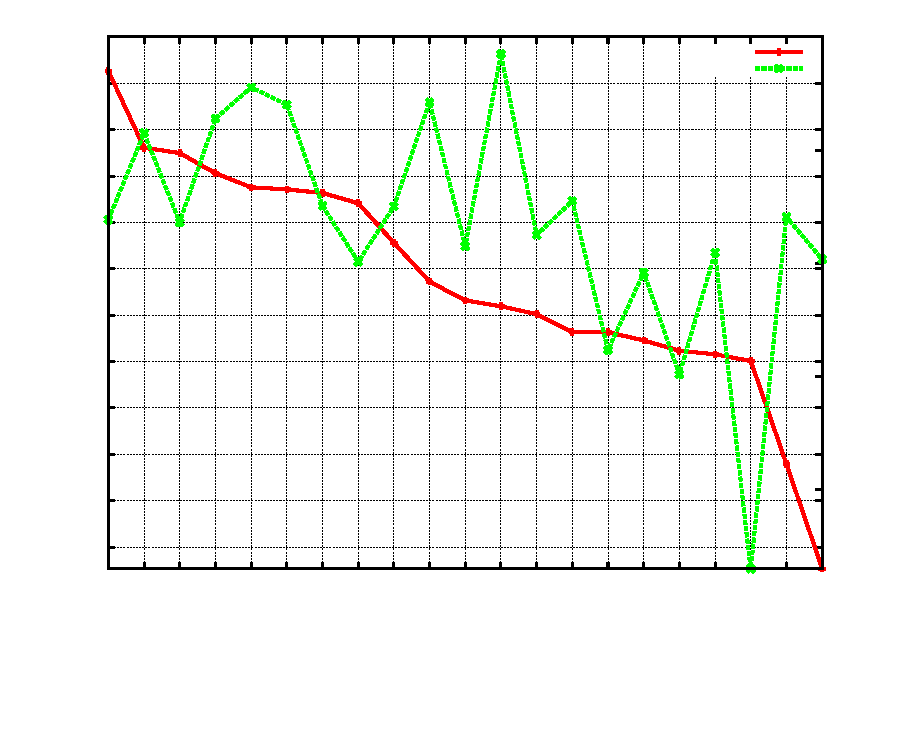
\includegraphics{plots/sent3}}%
    \gplfronttext
  \end{picture}%
\endgroup
}
  \scalebox{0.5}{% GNUPLOT: LaTeX picture with Postscript
\begingroup
  \makeatletter
  \providecommand\color[2][]{%
    \GenericError{(gnuplot) \space\space\space\@spaces}{%
      Package color not loaded in conjunction with
      terminal option `colourtext'%
    }{See the gnuplot documentation for explanation.%
    }{Either use 'blacktext' in gnuplot or load the package
      color.sty in LaTeX.}%
    \renewcommand\color[2][]{}%
  }%
  \providecommand\includegraphics[2][]{%
    \GenericError{(gnuplot) \space\space\space\@spaces}{%
      Package graphicx or graphics not loaded%
    }{See the gnuplot documentation for explanation.%
    }{The gnuplot epslatex terminal needs graphicx.sty or graphics.sty.}%
    \renewcommand\includegraphics[2][]{}%
  }%
  \providecommand\rotatebox[2]{#2}%
  \@ifundefined{ifGPcolor}{%
    \newif\ifGPcolor
    \GPcolortrue
  }{}%
  \@ifundefined{ifGPblacktext}{%
    \newif\ifGPblacktext
    \GPblacktexttrue
  }{}%
  % define a \g@addto@macro without @ in the name:
  \let\gplgaddtomacro\g@addto@macro
  % define empty templates for all commands taking text:
  \gdef\gplbacktext{}%
  \gdef\gplfronttext{}%
  \makeatother
  \ifGPblacktext
    % no textcolor at all
    \def\colorrgb#1{}%
    \def\colorgray#1{}%
  \else
    % gray or color?
    \ifGPcolor
      \def\colorrgb#1{\color[rgb]{#1}}%
      \def\colorgray#1{\color[gray]{#1}}%
      \expandafter\def\csname LTw\endcsname{\color{white}}%
      \expandafter\def\csname LTb\endcsname{\color{black}}%
      \expandafter\def\csname LTa\endcsname{\color{black}}%
      \expandafter\def\csname LT0\endcsname{\color[rgb]{1,0,0}}%
      \expandafter\def\csname LT1\endcsname{\color[rgb]{0,1,0}}%
      \expandafter\def\csname LT2\endcsname{\color[rgb]{0,0,1}}%
      \expandafter\def\csname LT3\endcsname{\color[rgb]{1,0,1}}%
      \expandafter\def\csname LT4\endcsname{\color[rgb]{0,1,1}}%
      \expandafter\def\csname LT5\endcsname{\color[rgb]{1,1,0}}%
      \expandafter\def\csname LT6\endcsname{\color[rgb]{0,0,0}}%
      \expandafter\def\csname LT7\endcsname{\color[rgb]{1,0.3,0}}%
      \expandafter\def\csname LT8\endcsname{\color[rgb]{0.5,0.5,0.5}}%
    \else
      % gray
      \def\colorrgb#1{\color{black}}%
      \def\colorgray#1{\color[gray]{#1}}%
      \expandafter\def\csname LTw\endcsname{\color{white}}%
      \expandafter\def\csname LTb\endcsname{\color{black}}%
      \expandafter\def\csname LTa\endcsname{\color{black}}%
      \expandafter\def\csname LT0\endcsname{\color{black}}%
      \expandafter\def\csname LT1\endcsname{\color{black}}%
      \expandafter\def\csname LT2\endcsname{\color{black}}%
      \expandafter\def\csname LT3\endcsname{\color{black}}%
      \expandafter\def\csname LT4\endcsname{\color{black}}%
      \expandafter\def\csname LT5\endcsname{\color{black}}%
      \expandafter\def\csname LT6\endcsname{\color{black}}%
      \expandafter\def\csname LT7\endcsname{\color{black}}%
      \expandafter\def\csname LT8\endcsname{\color{black}}%
    \fi
  \fi
  \setlength{\unitlength}{0.0500bp}%
  \begin{picture}(8502.00,6802.00)%
    \gplgaddtomacro\gplbacktext{%
      \csname LTb\endcsname%
      \put(784,2001){\makebox(0,0)[r]{\strut{} 98}}%
      \csname LTb\endcsname%
      \put(784,3153){\makebox(0,0)[r]{\strut{} 98.5}}%
      \csname LTb\endcsname%
      \put(784,4305){\makebox(0,0)[r]{\strut{} 99}}%
      \csname LTb\endcsname%
      \put(784,5457){\makebox(0,0)[r]{\strut{} 99.5}}%
      \csname LTb\endcsname%
      \put(784,6609){\makebox(0,0)[r]{\strut{} 100}}%
      \csname LTb\endcsname%
      \put(880,1408){\rotatebox{-270}{\makebox(0,0)[r]{\strut{}\relu}}}%
      \csname LTb\endcsname%
      \put(1223,1408){\rotatebox{-270}{\makebox(0,0)[r]{\strut{}\lrelua}}}%
      \csname LTb\endcsname%
      \put(1565,1408){\rotatebox{-270}{\makebox(0,0)[r]{\strut{}\maxoutc}}}%
      \csname LTb\endcsname%
      \put(1908,1408){\rotatebox{-270}{\makebox(0,0)[r]{\strut{}\maxoutb}}}%
      \csname LTb\endcsname%
      \put(2251,1408){\rotatebox{-270}{\makebox(0,0)[r]{\strut{}\pentan}}}%
      \csname LTb\endcsname%
      \put(2593,1408){\rotatebox{-270}{\makebox(0,0)[r]{\strut{}\prelu}}}%
      \csname LTb\endcsname%
      \put(2936,1408){\rotatebox{-270}{\makebox(0,0)[r]{\strut{}\maxouta}}}%
      \csname LTb\endcsname%
      \put(3279,1408){\rotatebox{-270}{\makebox(0,0)[r]{\strut{}\minsin}}}%
      \csname LTb\endcsname%
      \put(3621,1408){\rotatebox{-270}{\makebox(0,0)[r]{\strut{}\swish}}}%
      \csname LTb\endcsname%
      \put(3964,1408){\rotatebox{-270}{\makebox(0,0)[r]{\strut{}\mytanh}}}%
      \csname LTb\endcsname%
      \put(4307,1408){\rotatebox{-270}{\makebox(0,0)[r]{\strut{}\selu}}}%
      \csname LTb\endcsname%
      \put(4649,1408){\rotatebox{-270}{\makebox(0,0)[r]{\strut{}\mysin}}}%
      \csname LTb\endcsname%
      \put(4992,1408){\rotatebox{-270}{\makebox(0,0)[r]{\strut{}\lrelub}}}%
      \csname LTb\endcsname%
      \put(5334,1408){\rotatebox{-270}{\makebox(0,0)[r]{\strut{}\maxsig}}}%
      \csname LTb\endcsname%
      \put(5677,1408){\rotatebox{-270}{\makebox(0,0)[r]{\strut{}\maxtanh}}}%
      \csname LTb\endcsname%
      \put(6020,1408){\rotatebox{-270}{\makebox(0,0)[r]{\strut{}\cosid}}}%
      \csname LTb\endcsname%
      \put(6362,1408){\rotatebox{-270}{\makebox(0,0)[r]{\strut{}\cube}}}%
      \csname LTb\endcsname%
      \put(6705,1408){\rotatebox{-270}{\makebox(0,0)[r]{\strut{}\sigmoid}}}%
      \csname LTb\endcsname%
      \put(7048,1408){\rotatebox{-270}{\makebox(0,0)[r]{\strut{}\arctid}}}%
      \csname LTb\endcsname%
      \put(7390,1408){\rotatebox{-270}{\makebox(0,0)[r]{\strut{}\elu}}}%
      \csname LTb\endcsname%
      \put(7733,1408){\rotatebox{-270}{\makebox(0,0)[r]{\strut{}\linear}}}%
      \put(7829,2103){\makebox(0,0)[l]{\strut{} 69}}%
      \put(7829,2830){\makebox(0,0)[l]{\strut{} 74}}%
      \put(7829,3557){\makebox(0,0)[l]{\strut{} 79}}%
      \put(7829,4284){\makebox(0,0)[l]{\strut{} 84}}%
      \put(7829,5010){\makebox(0,0)[l]{\strut{} 89}}%
      \put(7829,5737){\makebox(0,0)[l]{\strut{} 94}}%
      \put(7829,6464){\makebox(0,0)[l]{\strut{} 99}}%
      \put(128,4056){\rotatebox{-270}{\makebox(0,0){\strut{}Score}}}%
    }%
    \gplgaddtomacro\gplfronttext{%
      \csname LTb\endcsname%
      \put(6998,6466){\makebox(0,0)[r]{\strut{}\best{}}}%
      \csname LTb\endcsname%
      \put(6998,6306){\makebox(0,0)[r]{\strut{}\avg{}}}%
    }%
    \gplbacktext
    \put(0,0){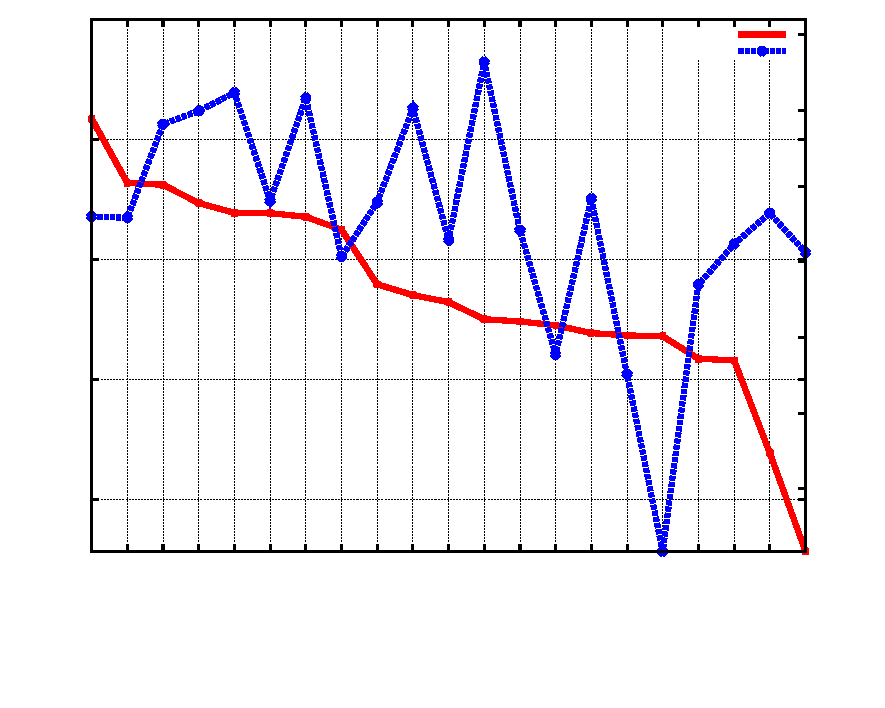
\includegraphics{plots/sent-X.pdf}}%
    \gplfronttext
  \end{picture}%
\endgroup
}
  \caption{Sentence Classification. Left y-axis: \best. Right y-axis: \avg{}. Score on y-axes is the average over all mini-experiments.}
  \label{fig:sent}
\end{figure}

\avg{} results are very different from \best{} results. Here, somewhat surprisingly, the oscillating \mysin{} function wins, followed by \pentan{}, maxout and \swish. The difference between the best \avg{} function, \mysin, and the worst, \cube, is more than 30pp. This means that using \cube{} is much riskier and requires more careful hyperparameter search compared to \mysin{} and the other top performers. 
%Figure \ref{fig:sent} also shows that better \best{} performers tend to be better \avg{} performers, and vice versa. 
%have better average performance and vice versa. 

\subsection{CNN \& Document Classification}\label{sec:2}
\paragraph{Model} Our second paradigm is document classification using a CNN. This approach has been popularized in NLP by the ground-breaking work of \citet{Kim:2014}. Even though shallow CNNs do not reach state-of-the-art results on large datasets anymore \cite{Johnson:2017}, simple approaches like (shallow) CNNs are still very competitive for smaller datasets \cite{Joulin:2016}. 

Our model operates on token-level and first embeds a sequence of tokens $x_1,\ldots,x_n$, represented as 1-hot vectors, into learnable embeddings $\mathbf{x}_1,\ldots,\mathbf{x}_n$. The model then applies 1D-convolution on top of these embeddings. That is, a filter $\mathbf{w}$ of size $h$ takes $h$ successive embeddings $\mathbf{x}_{i:i+h-1}$, performs a scalar product and obtains a feature $c_i$:
\begin{align*}
  c_i = f(\mathbf{w}\cdot \mathbf{x}_{i:i+h-1}+b).
\end{align*}
Here, $f$ is the activation function and $b$ is a bias term. We take the number $n_k$ of different filters as a hyperparameter. When our network has multiple layers, we stack another convolutional layer on top of the first (in total we have $n_k$ outputs at each time step), and so on. Our penultimate layer is a global max pooling layers that selects the maximum from each feature map. A final softmax layer terminates the network. 
\paragraph{Data} We use two document classification tasks, namely: 20 Newsgroup (NG) and Reuters-21578 R8 (R8). Both datasets are standard document classification datasets. In NG, the goal is to classify each document into one of 20 newsgroup classes (alt.atheism, sci.med, sci.space, etc.). In R8, the goal is to classify Reuters news text into one of eight classes (crude, earn, grain, interest, etc.).  We used the preprocessed files from \url{https://www.cs.umb.edu/~smimarog/textmining/datasets/} (in particular, stopwords are removed and the text is stemmed).
\paragraph{Approach}
We consider 4 mini-experiments:
\begin{itemize}[noitemsep,leftmargin=0.6cm]
\item (1,2) NG dataset with 5\% and 50\%, respectively of the full data as train data. In both cases, 10\% of the full data is used as dev data, and the rest as test data.  
\item (3,4) Same as (1,2) for R8. 
%R8 dataset with same specifications as for NG.
\end{itemize}
We report accuracy for all experiments. We use a batch size of 64, 50 epochs for training, and a patience of 10. For all mini-experiments, we again draw 200 randomly chosen hyperparameters from the ranges indicated in Table \ref{table:hyperparams_sent}. 
%As for the train/dev/test splits, 
The hyperparameters and train/dev/test splits are the same for all activation functions. 

\paragraph{Results}
Figure \ref{fig:doc} shows \best{} and \avg{} results, averaged over all mini-experiments. This time, the winners for \best{} are \elu{}, \selu{} (again two members from the rectifier family), and \maxoutb{}, but the difference between \maxoutb{} and several lower ranked functions is minimal. The \cube{} function is again worst and \sigmoid{} and \cosid{} have similarly bad performance. Except for \minsin{}, the newly proposed activation functions from \citet{Ramach:2018} again considerably lag behind. The most stable activation functions are the maxout functions as well as \pentan{}, \mytanh{} and \mysin{}.  

\begin{figure}[!htb]
\centering
%\scalebox{0.5}{% GNUPLOT: LaTeX picture with Postscript
\begingroup
  \makeatletter
  \providecommand\color[2][]{%
    \GenericError{(gnuplot) \space\space\space\@spaces}{%
      Package color not loaded in conjunction with
      terminal option `colourtext'%
    }{See the gnuplot documentation for explanation.%
    }{Either use 'blacktext' in gnuplot or load the package
      color.sty in LaTeX.}%
    \renewcommand\color[2][]{}%
  }%
  \providecommand\includegraphics[2][]{%
    \GenericError{(gnuplot) \space\space\space\@spaces}{%
      Package graphicx or graphics not loaded%
    }{See the gnuplot documentation for explanation.%
    }{The gnuplot epslatex terminal needs graphicx.sty or graphics.sty.}%
    \renewcommand\includegraphics[2][]{}%
  }%
  \providecommand\rotatebox[2]{#2}%
  \@ifundefined{ifGPcolor}{%
    \newif\ifGPcolor
    \GPcolortrue
  }{}%
  \@ifundefined{ifGPblacktext}{%
    \newif\ifGPblacktext
    \GPblacktexttrue
  }{}%
  % define a \g@addto@macro without @ in the name:
  \let\gplgaddtomacro\g@addto@macro
  % define empty templates for all commands taking text:
  \gdef\gplbacktext{}%
  \gdef\gplfronttext{}%
  \makeatother
  \ifGPblacktext
    % no textcolor at all
    \def\colorrgb#1{}%
    \def\colorgray#1{}%
  \else
    % gray or color?
    \ifGPcolor
      \def\colorrgb#1{\color[rgb]{#1}}%
      \def\colorgray#1{\color[gray]{#1}}%
      \expandafter\def\csname LTw\endcsname{\color{white}}%
      \expandafter\def\csname LTb\endcsname{\color{black}}%
      \expandafter\def\csname LTa\endcsname{\color{black}}%
      \expandafter\def\csname LT0\endcsname{\color[rgb]{1,0,0}}%
      \expandafter\def\csname LT1\endcsname{\color[rgb]{0,1,0}}%
      \expandafter\def\csname LT2\endcsname{\color[rgb]{0,0,1}}%
      \expandafter\def\csname LT3\endcsname{\color[rgb]{1,0,1}}%
      \expandafter\def\csname LT4\endcsname{\color[rgb]{0,1,1}}%
      \expandafter\def\csname LT5\endcsname{\color[rgb]{1,1,0}}%
      \expandafter\def\csname LT6\endcsname{\color[rgb]{0,0,0}}%
      \expandafter\def\csname LT7\endcsname{\color[rgb]{1,0.3,0}}%
      \expandafter\def\csname LT8\endcsname{\color[rgb]{0.5,0.5,0.5}}%
    \else
      % gray
      \def\colorrgb#1{\color{black}}%
      \def\colorgray#1{\color[gray]{#1}}%
      \expandafter\def\csname LTw\endcsname{\color{white}}%
      \expandafter\def\csname LTb\endcsname{\color{black}}%
      \expandafter\def\csname LTa\endcsname{\color{black}}%
      \expandafter\def\csname LT0\endcsname{\color{black}}%
      \expandafter\def\csname LT1\endcsname{\color{black}}%
      \expandafter\def\csname LT2\endcsname{\color{black}}%
      \expandafter\def\csname LT3\endcsname{\color{black}}%
      \expandafter\def\csname LT4\endcsname{\color{black}}%
      \expandafter\def\csname LT5\endcsname{\color{black}}%
      \expandafter\def\csname LT6\endcsname{\color{black}}%
      \expandafter\def\csname LT7\endcsname{\color{black}}%
      \expandafter\def\csname LT8\endcsname{\color{black}}%
    \fi
  \fi
  \setlength{\unitlength}{0.0500bp}%
  \begin{picture}(8502.00,6802.00)%
    \gplgaddtomacro\gplbacktext{%
      \csname LTb\endcsname%
      \put(784,1687){\makebox(0,0)[r]{\strut{} 79}}%
      \csname LTb\endcsname%
      \put(784,1960){\makebox(0,0)[r]{\strut{} 79.2}}%
      \csname LTb\endcsname%
      \put(784,2234){\makebox(0,0)[r]{\strut{} 79.4}}%
      \csname LTb\endcsname%
      \put(784,2507){\makebox(0,0)[r]{\strut{} 79.6}}%
      \csname LTb\endcsname%
      \put(784,2781){\makebox(0,0)[r]{\strut{} 79.8}}%
      \csname LTb\endcsname%
      \put(784,3054){\makebox(0,0)[r]{\strut{} 80}}%
      \csname LTb\endcsname%
      \put(784,3328){\makebox(0,0)[r]{\strut{} 80.2}}%
      \csname LTb\endcsname%
      \put(784,3601){\makebox(0,0)[r]{\strut{} 80.4}}%
      \csname LTb\endcsname%
      \put(784,3875){\makebox(0,0)[r]{\strut{} 80.6}}%
      \csname LTb\endcsname%
      \put(784,4148){\makebox(0,0)[r]{\strut{} 80.8}}%
      \csname LTb\endcsname%
      \put(784,4421){\makebox(0,0)[r]{\strut{} 81}}%
      \csname LTb\endcsname%
      \put(784,4695){\makebox(0,0)[r]{\strut{} 81.2}}%
      \csname LTb\endcsname%
      \put(784,4968){\makebox(0,0)[r]{\strut{} 81.4}}%
      \csname LTb\endcsname%
      \put(784,5242){\makebox(0,0)[r]{\strut{} 81.6}}%
      \csname LTb\endcsname%
      \put(784,5515){\makebox(0,0)[r]{\strut{} 81.8}}%
      \csname LTb\endcsname%
      \put(784,5789){\makebox(0,0)[r]{\strut{} 82}}%
      \csname LTb\endcsname%
      \put(784,6062){\makebox(0,0)[r]{\strut{} 82.2}}%
      \csname LTb\endcsname%
      \put(784,6336){\makebox(0,0)[r]{\strut{} 82.4}}%
      \csname LTb\endcsname%
      \put(784,6609){\makebox(0,0)[r]{\strut{} 82.6}}%
      \csname LTb\endcsname%
      \put(880,1408){\rotatebox{-270}{\makebox(0,0)[r]{\strut{}elu}}}%
      \csname LTb\endcsname%
      \put(1223,1408){\rotatebox{-270}{\makebox(0,0)[r]{\strut{}selu}}}%
      \csname LTb\endcsname%
      \put(1565,1408){\rotatebox{-270}{\makebox(0,0)[r]{\strut{}tanh}}}%
      \csname LTb\endcsname%
      \put(1908,1408){\rotatebox{-270}{\makebox(0,0)[r]{\strut{}minsin}}}%
      \csname LTb\endcsname%
      \put(2251,1408){\rotatebox{-270}{\makebox(0,0)[r]{\strut{}maxout-2}}}%
      \csname LTb\endcsname%
      \put(2593,1408){\rotatebox{-270}{\makebox(0,0)[r]{\strut{}penalized\_tanh}}}%
      \csname LTb\endcsname%
      \put(2936,1408){\rotatebox{-270}{\makebox(0,0)[r]{\strut{}maxout-3}}}%
      \csname LTb\endcsname%
      \put(3279,1408){\rotatebox{-270}{\makebox(0,0)[r]{\strut{}sin}}}%
      \csname LTb\endcsname%
      \put(3621,1408){\rotatebox{-270}{\makebox(0,0)[r]{\strut{}maxout-4}}}%
      \csname LTb\endcsname%
      \put(3964,1408){\rotatebox{-270}{\makebox(0,0)[r]{\strut{}prelu}}}%
      \csname LTb\endcsname%
      \put(4307,1408){\rotatebox{-270}{\makebox(0,0)[r]{\strut{}leakyrelu-0.3}}}%
      \csname LTb\endcsname%
      \put(4649,1408){\rotatebox{-270}{\makebox(0,0)[r]{\strut{}linear}}}%
      \csname LTb\endcsname%
      \put(4992,1408){\rotatebox{-270}{\makebox(0,0)[r]{\strut{}maxtanh}}}%
      \csname LTb\endcsname%
      \put(5334,1408){\rotatebox{-270}{\makebox(0,0)[r]{\strut{}leakyrelu-0.01}}}%
      \csname LTb\endcsname%
      \put(5677,1408){\rotatebox{-270}{\makebox(0,0)[r]{\strut{}relu}}}%
      \csname LTb\endcsname%
      \put(6020,1408){\rotatebox{-270}{\makebox(0,0)[r]{\strut{}tanhrev}}}%
      \csname LTb\endcsname%
      \put(6362,1408){\rotatebox{-270}{\makebox(0,0)[r]{\strut{}swish}}}%
      \csname LTb\endcsname%
      \put(6705,1408){\rotatebox{-270}{\makebox(0,0)[r]{\strut{}cosper}}}%
      \csname LTb\endcsname%
      \put(7048,1408){\rotatebox{-270}{\makebox(0,0)[r]{\strut{}sigmoid}}}%
      \csname LTb\endcsname%
      \put(7390,1408){\rotatebox{-270}{\makebox(0,0)[r]{\strut{}maxsig}}}%
      \csname LTb\endcsname%
      \put(7733,1408){\rotatebox{-270}{\makebox(0,0)[r]{\strut{}cube}}}%
      \put(7829,2171){\makebox(0,0)[l]{\strut{} 45}}%
      \put(7829,3059){\makebox(0,0)[l]{\strut{} 50}}%
      \put(7829,3946){\makebox(0,0)[l]{\strut{} 55}}%
      \put(7829,4834){\makebox(0,0)[l]{\strut{} 60}}%
      \put(7829,5721){\makebox(0,0)[l]{\strut{} 65}}%
      \put(7829,6609){\makebox(0,0)[l]{\strut{} 70}}%
      \csname LTb\endcsname%
      \put(128,4056){\rotatebox{-270}{\makebox(0,0){\strut{}Score}}}%
    }%
    \gplgaddtomacro\gplfronttext{%
      \csname LTb\endcsname%
      \put(6998,1807){\makebox(0,0)[r]{\strut{}Best}}%
      \csname LTb\endcsname%
      \put(6998,1647){\makebox(0,0)[r]{\strut{}Avg}}%
    }%
    \gplbacktext
    \put(0,0){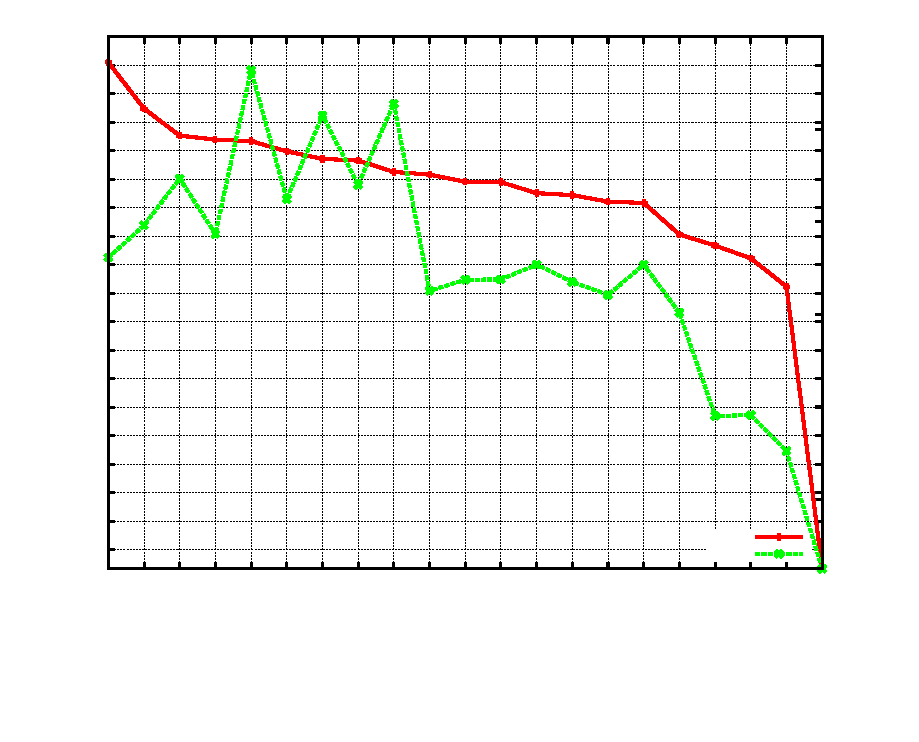
\includegraphics{plots/doc2}}%
    \gplfronttext
  \end{picture}%
\endgroup
}
\scalebox{0.5}{% GNUPLOT: LaTeX picture with Postscript
\begingroup
  \makeatletter
  \providecommand\color[2][]{%
    \GenericError{(gnuplot) \space\space\space\@spaces}{%
      Package color not loaded in conjunction with
      terminal option `colourtext'%
    }{See the gnuplot documentation for explanation.%
    }{Either use 'blacktext' in gnuplot or load the package
      color.sty in LaTeX.}%
    \renewcommand\color[2][]{}%
  }%
  \providecommand\includegraphics[2][]{%
    \GenericError{(gnuplot) \space\space\space\@spaces}{%
      Package graphicx or graphics not loaded%
    }{See the gnuplot documentation for explanation.%
    }{The gnuplot epslatex terminal needs graphicx.sty or graphics.sty.}%
    \renewcommand\includegraphics[2][]{}%
  }%
  \providecommand\rotatebox[2]{#2}%
  \@ifundefined{ifGPcolor}{%
    \newif\ifGPcolor
    \GPcolortrue
  }{}%
  \@ifundefined{ifGPblacktext}{%
    \newif\ifGPblacktext
    \GPblacktexttrue
  }{}%
  % define a \g@addto@macro without @ in the name:
  \let\gplgaddtomacro\g@addto@macro
  % define empty templates for all commands taking text:
  \gdef\gplbacktext{}%
  \gdef\gplfronttext{}%
  \makeatother
  \ifGPblacktext
    % no textcolor at all
    \def\colorrgb#1{}%
    \def\colorgray#1{}%
  \else
    % gray or color?
    \ifGPcolor
      \def\colorrgb#1{\color[rgb]{#1}}%
      \def\colorgray#1{\color[gray]{#1}}%
      \expandafter\def\csname LTw\endcsname{\color{white}}%
      \expandafter\def\csname LTb\endcsname{\color{black}}%
      \expandafter\def\csname LTa\endcsname{\color{black}}%
      \expandafter\def\csname LT0\endcsname{\color[rgb]{1,0,0}}%
      \expandafter\def\csname LT1\endcsname{\color[rgb]{0,1,0}}%
      \expandafter\def\csname LT2\endcsname{\color[rgb]{0,0,1}}%
      \expandafter\def\csname LT3\endcsname{\color[rgb]{1,0,1}}%
      \expandafter\def\csname LT4\endcsname{\color[rgb]{0,1,1}}%
      \expandafter\def\csname LT5\endcsname{\color[rgb]{1,1,0}}%
      \expandafter\def\csname LT6\endcsname{\color[rgb]{0,0,0}}%
      \expandafter\def\csname LT7\endcsname{\color[rgb]{1,0.3,0}}%
      \expandafter\def\csname LT8\endcsname{\color[rgb]{0.5,0.5,0.5}}%
    \else
      % gray
      \def\colorrgb#1{\color{black}}%
      \def\colorgray#1{\color[gray]{#1}}%
      \expandafter\def\csname LTw\endcsname{\color{white}}%
      \expandafter\def\csname LTb\endcsname{\color{black}}%
      \expandafter\def\csname LTa\endcsname{\color{black}}%
      \expandafter\def\csname LT0\endcsname{\color{black}}%
      \expandafter\def\csname LT1\endcsname{\color{black}}%
      \expandafter\def\csname LT2\endcsname{\color{black}}%
      \expandafter\def\csname LT3\endcsname{\color{black}}%
      \expandafter\def\csname LT4\endcsname{\color{black}}%
      \expandafter\def\csname LT5\endcsname{\color{black}}%
      \expandafter\def\csname LT6\endcsname{\color{black}}%
      \expandafter\def\csname LT7\endcsname{\color{black}}%
      \expandafter\def\csname LT8\endcsname{\color{black}}%
    \fi
  \fi
  \setlength{\unitlength}{0.0500bp}%
  \begin{picture}(8502.00,6802.00)%
    \gplgaddtomacro\gplbacktext{%
      \csname LTb\endcsname%
      \put(784,1551){\makebox(0,0)[r]{\strut{} 94.5}}%
      \csname LTb\endcsname%
      \put(784,2010){\makebox(0,0)[r]{\strut{} 95}}%
      \csname LTb\endcsname%
      \put(784,2470){\makebox(0,0)[r]{\strut{} 95.5}}%
      \csname LTb\endcsname%
      \put(784,2930){\makebox(0,0)[r]{\strut{} 96}}%
      \csname LTb\endcsname%
      \put(784,3390){\makebox(0,0)[r]{\strut{} 96.5}}%
      \csname LTb\endcsname%
      \put(784,3850){\makebox(0,0)[r]{\strut{} 97}}%
      \csname LTb\endcsname%
      \put(784,4310){\makebox(0,0)[r]{\strut{} 97.5}}%
      \csname LTb\endcsname%
      \put(784,4770){\makebox(0,0)[r]{\strut{} 98}}%
      \csname LTb\endcsname%
      \put(784,5229){\makebox(0,0)[r]{\strut{} 98.5}}%
      \csname LTb\endcsname%
      \put(784,5689){\makebox(0,0)[r]{\strut{} 99}}%
      \csname LTb\endcsname%
      \put(784,6149){\makebox(0,0)[r]{\strut{} 99.5}}%
      \csname LTb\endcsname%
      \put(784,6609){\makebox(0,0)[r]{\strut{} 100}}%
      \csname LTb\endcsname%
      \put(880,1408){\rotatebox{-270}{\makebox(0,0)[r]{\strut{}\elu}}}%
      \csname LTb\endcsname%
      \put(1218,1408){\rotatebox{-270}{\makebox(0,0)[r]{\strut{}\selu}}}%
      \csname LTb\endcsname%
      \put(1556,1408){\rotatebox{-270}{\makebox(0,0)[r]{\strut{}\maxouta}}}%
      \csname LTb\endcsname%
      \put(1894,1408){\rotatebox{-270}{\makebox(0,0)[r]{\strut{}\mytanh}}}%
      \csname LTb\endcsname%
      \put(2231,1408){\rotatebox{-270}{\makebox(0,0)[r]{\strut{}\minsin}}}%
      \csname LTb\endcsname%
      \put(2569,1408){\rotatebox{-270}{\makebox(0,0)[r]{\strut{}\pentan}}}%
      \csname LTb\endcsname%
      \put(2907,1408){\rotatebox{-270}{\makebox(0,0)[r]{\strut{}\maxoutb}}}%
      \csname LTb\endcsname%
      \put(3245,1408){\rotatebox{-270}{\makebox(0,0)[r]{\strut{}\mysin}}}%
      \csname LTb\endcsname%
      \put(3583,1408){\rotatebox{-270}{\makebox(0,0)[r]{\strut{}\maxoutc}}}%
      \csname LTb\endcsname%
      \put(3921,1408){\rotatebox{-270}{\makebox(0,0)[r]{\strut{}\prelu}}}%
      \csname LTb\endcsname%
      \put(4259,1408){\rotatebox{-270}{\makebox(0,0)[r]{\strut{}\linear}}}%
      \csname LTb\endcsname%
      \put(4596,1408){\rotatebox{-270}{\makebox(0,0)[r]{\strut{}\lrelub}}}%
      \csname LTb\endcsname%
      \put(4934,1408){\rotatebox{-270}{\makebox(0,0)[r]{\strut{}\maxtanh}}}%
      \csname LTb\endcsname%
      \put(5272,1408){\rotatebox{-270}{\makebox(0,0)[r]{\strut{}\lrelua}}}%
      \csname LTb\endcsname%
      \put(5610,1408){\rotatebox{-270}{\makebox(0,0)[r]{\strut{}\relu}}}%
      \csname LTb\endcsname%
      \put(5948,1408){\rotatebox{-270}{\makebox(0,0)[r]{\strut{}\arctid}}}%
      \csname LTb\endcsname%
      \put(6286,1408){\rotatebox{-270}{\makebox(0,0)[r]{\strut{}\cosid}}}%
      \csname LTb\endcsname%
      \put(6623,1408){\rotatebox{-270}{\makebox(0,0)[r]{\strut{}\sigmoid}}}%
      \csname LTb\endcsname%
      \put(6961,1408){\rotatebox{-270}{\makebox(0,0)[r]{\strut{}\swish}}}%
      \csname LTb\endcsname%
      \put(7299,1408){\rotatebox{-270}{\makebox(0,0)[r]{\strut{}\maxsig}}}%
      \csname LTb\endcsname%
      \put(7637,1408){\rotatebox{-270}{\makebox(0,0)[r]{\strut{}\cube}}}%
      \put(7733,1992){\makebox(0,0)[l]{\strut{} 60}}%
      \put(7733,2569){\makebox(0,0)[l]{\strut{} 65}}%
      \put(7733,3146){\makebox(0,0)[l]{\strut{} 70}}%
      \put(7733,3723){\makebox(0,0)[l]{\strut{} 75}}%
      \put(7733,4300){\makebox(0,0)[l]{\strut{} 80}}%
      \put(7733,4878){\makebox(0,0)[l]{\strut{} 85}}%
      \put(7733,5455){\makebox(0,0)[l]{\strut{} 90}}%
      \put(7733,6032){\makebox(0,0)[l]{\strut{} 95}}%
      \put(7733,6609){\makebox(0,0)[l]{\strut{} 100}}%
      \put(128,4056){\rotatebox{-270}{\makebox(0,0){\strut{}Score}}}%
    }%
    \gplgaddtomacro\gplfronttext{%
      \csname LTb\endcsname%
      \put(6902,6466){\makebox(0,0)[r]{\strut{}\best}}%
      \csname LTb\endcsname%
      \put(6902,6306){\makebox(0,0)[r]{\strut{}\avg}}%
    }%
    \gplbacktext
    \put(0,0){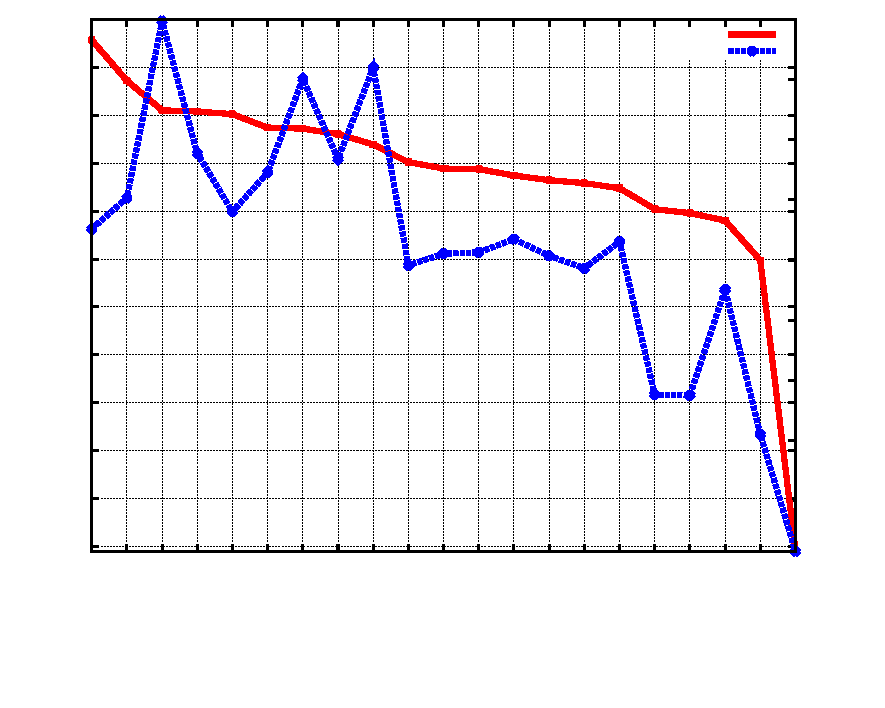
\includegraphics{plots/doc-X.pdf}}%
    \gplfronttext
  \end{picture}%
\endgroup
}
\caption{Doc classification.}
\label{fig:doc}
\end{figure}

\subsection{RNN \& Sequence Tagging}\label{sec:3}
\paragraph{Model} Our third paradigm is sequence tagging, a ubiquitous model type in NLP. In sequence tagging, a sequence of input tokens $w_1,\ldots,w_K$ is mapped to a sequence of labels $y_1,\ldots,y_K$. Classical sequence tagging tasks include POS tagging, chunking, NER, discourse parsing \cite{Braud:2017}, and argumentation mining \cite{Eger:2017,Schulz:2018}. We use a standard recurrent net for sequence tagging, whose form is:
\begin{align*}
  \mathbf{h}_i &= f(\mathbf{h}_{i-1}\mathbf{W}+\mathbf{w}_i\cdot\mathbf{U}+\mathbf{b})\\
  \mathbf{y}_i &= \text{softmax}(\mathbf{h}_i\mathbf{V}+\mathbf{c})
\end{align*}
Here, $\mathbf{w}_i$ are (pre-trained) word embeddings of words $w_i$. Vectors $\mathbf{b},\mathbf{c}$ and matrices $\mathbf{U},\mathbf{V},\mathbf{W}$ are parameters to be learned during training. The above describes an RNN with only one hidden layer, $\mathbf{h}_i$, at each time step, but we consider the generalized form with $N\ge 1$ hidden layers; we also choose a bidirectional RNN in which the hidden outputs of a forward RNN and a backward RNN are combined. 
RNNs are particularly deep networks---indeed, the depth of the network corresponds to the length of the input sequence---which makes them particularly susceptible to the vanishing gradient problem \cite{Pascanu:2013}. 

%[Say a word on LSTMs]
Initially, we do not consider the more popular LSTMs here for reasons indicated below. However, we include a comparison after discussing the RNN performance. 
%for two reasons: (i) activation functions in LSTMs usually take other roles than in standard RNNs, namely, that of gating (gate is open, closed, or in-between), and thus, the expectation is that the choice of activation function is either not as important or restricted to certain `binary-like' function; (ii) with proper initialization, standard RNNs have been shown to be able to perform as well, or even better, than LSTMs \cite{Le:2015}. However, we will also compare RNNs to LSTMs, albeit in fewer scenarios. 

\paragraph{Data}
We use two sequence tagging tasks, namely: English POS tagging (POS), and token-level argumentation mining (TL-AM) using the same dataset (consisting of student essays) as for the sentence level experiments. In token-level AM, we tag each token with a BIO-label plus the component type, i.e., the label space is $\mathcal{Y}=\{\text{B},\text{I}\}\times\{\text{MC},\text{C},\text{P}\}\cup\{\text{O}\}$, where 
%MC stands for major claim, C for claim, and P for premise, and `
`O'' is a label for non-argumentative tokens. The motivation for using TL-AM is that, putatively, AM has more long-range dependencies than POS or similar sequence tagging tasks such as NER, because argument components are much longer than named entities and component labels also %do not 
depend less %very much 
on the current token.  

%Dataset statistics are shown in Table \ref{table:data_sent}. 
\paragraph{Approach} We consider 6 mini-experiments: 
\begin{itemize}[noitemsep,leftmargin=0.6cm]
  \item (1): TL-AM with Glove-100d word embeddings and 5\% of the original training data as train data; (2) the same with 30\% of the original training data as train data. In both cases, dev and test follow the original train splits \cite{Eger:2017}. 
  \item (3,4) Same as (1) and (2) but with 300d Levy word embeddings \cite{Levy:2014}.
  \item (5,6): POS with Glove-100d word embeddings and 5\% and 30\%, respectively, of the train data of a pre-determined train/dev/test split (13k/13k/178k tokens). Dev and test are fixed in both cases.    
\end{itemize}
We report macro-F1 for mini-experiments (1-4) and accuracy for (5-6). For our RNN implementations, we use the accompanying code of (the state-of-the-art model of) \citet{Reimers:2017}, which is implemented in keras. The network uses a CRF layer as an output layer. We use a batch size of 32, train for 50 epochs and use a patience of 5 for early stopping.
\paragraph{Results}
Figure \ref{fig:seq} shows \best{} and \avg{} results, averaged over all 6 mini-experiments, for each activation function. We exclude \prelu{} and the maxout functions because the keras implementation does not natively support these activation functions for RNNs. We also exclude the \cube{} function because it performed very badly.  \begin{figure}[!htb]
\centering
\scalebox{0.5}{
%% GNUPLOT: LaTeX picture with Postscript
\begingroup
  \makeatletter
  \providecommand\color[2][]{%
    \GenericError{(gnuplot) \space\space\space\@spaces}{%
      Package color not loaded in conjunction with
      terminal option `colourtext'%
    }{See the gnuplot documentation for explanation.%
    }{Either use 'blacktext' in gnuplot or load the package
      color.sty in LaTeX.}%
    \renewcommand\color[2][]{}%
  }%
  \providecommand\includegraphics[2][]{%
    \GenericError{(gnuplot) \space\space\space\@spaces}{%
      Package graphicx or graphics not loaded%
    }{See the gnuplot documentation for explanation.%
    }{The gnuplot epslatex terminal needs graphicx.sty or graphics.sty.}%
    \renewcommand\includegraphics[2][]{}%
  }%
  \providecommand\rotatebox[2]{#2}%
  \@ifundefined{ifGPcolor}{%
    \newif\ifGPcolor
    \GPcolortrue
  }{}%
  \@ifundefined{ifGPblacktext}{%
    \newif\ifGPblacktext
    \GPblacktexttrue
  }{}%
  % define a \g@addto@macro without @ in the name:
  \let\gplgaddtomacro\g@addto@macro
  % define empty templates for all commands taking text:
  \gdef\gplbacktext{}%
  \gdef\gplfronttext{}%
  \makeatother
  \ifGPblacktext
    % no textcolor at all
    \def\colorrgb#1{}%
    \def\colorgray#1{}%
  \else
    % gray or color?
    \ifGPcolor
      \def\colorrgb#1{\color[rgb]{#1}}%
      \def\colorgray#1{\color[gray]{#1}}%
      \expandafter\def\csname LTw\endcsname{\color{white}}%
      \expandafter\def\csname LTb\endcsname{\color{black}}%
      \expandafter\def\csname LTa\endcsname{\color{black}}%
      \expandafter\def\csname LT0\endcsname{\color[rgb]{1,0,0}}%
      \expandafter\def\csname LT1\endcsname{\color[rgb]{0,1,0}}%
      \expandafter\def\csname LT2\endcsname{\color[rgb]{0,0,1}}%
      \expandafter\def\csname LT3\endcsname{\color[rgb]{1,0,1}}%
      \expandafter\def\csname LT4\endcsname{\color[rgb]{0,1,1}}%
      \expandafter\def\csname LT5\endcsname{\color[rgb]{1,1,0}}%
      \expandafter\def\csname LT6\endcsname{\color[rgb]{0,0,0}}%
      \expandafter\def\csname LT7\endcsname{\color[rgb]{1,0.3,0}}%
      \expandafter\def\csname LT8\endcsname{\color[rgb]{0.5,0.5,0.5}}%
    \else
      % gray
      \def\colorrgb#1{\color{black}}%
      \def\colorgray#1{\color[gray]{#1}}%
      \expandafter\def\csname LTw\endcsname{\color{white}}%
      \expandafter\def\csname LTb\endcsname{\color{black}}%
      \expandafter\def\csname LTa\endcsname{\color{black}}%
      \expandafter\def\csname LT0\endcsname{\color{black}}%
      \expandafter\def\csname LT1\endcsname{\color{black}}%
      \expandafter\def\csname LT2\endcsname{\color{black}}%
      \expandafter\def\csname LT3\endcsname{\color{black}}%
      \expandafter\def\csname LT4\endcsname{\color{black}}%
      \expandafter\def\csname LT5\endcsname{\color{black}}%
      \expandafter\def\csname LT6\endcsname{\color{black}}%
      \expandafter\def\csname LT7\endcsname{\color{black}}%
      \expandafter\def\csname LT8\endcsname{\color{black}}%
    \fi
  \fi
  \setlength{\unitlength}{0.0500bp}%
  \begin{picture}(8502.00,6802.00)%
    \gplgaddtomacro\gplbacktext{%
      \csname LTb\endcsname%
      \put(592,2139){\makebox(0,0)[r]{\strut{} 51}}%
      \csname LTb\endcsname%
      \put(592,3256){\makebox(0,0)[r]{\strut{} 54}}%
      \csname LTb\endcsname%
      \put(592,4374){\makebox(0,0)[r]{\strut{} 57}}%
      \csname LTb\endcsname%
      \put(592,5491){\makebox(0,0)[r]{\strut{} 60}}%
      \csname LTb\endcsname%
      \put(592,6609){\makebox(0,0)[r]{\strut{} 63}}%
      \csname LTb\endcsname%
      \put(688,1408){\rotatebox{-270}{\makebox(0,0)[r]{\strut{}lrelu001}}}%
      \csname LTb\endcsname%
      \put(1158,1408){\rotatebox{-270}{\makebox(0,0)[r]{\strut{}relu}}}%
      \csname LTb\endcsname%
      \put(1627,1408){\rotatebox{-270}{\makebox(0,0)[r]{\strut{}swish}}}%
      \csname LTb\endcsname%
      \put(2097,1408){\rotatebox{-270}{\makebox(0,0)[r]{\strut{}penalized\_tanh}}}%
      \csname LTb\endcsname%
      \put(2567,1408){\rotatebox{-270}{\makebox(0,0)[r]{\strut{}lrelu030}}}%
      \csname LTb\endcsname%
      \put(3036,1408){\rotatebox{-270}{\makebox(0,0)[r]{\strut{}tanhrev}}}%
      \csname LTb\endcsname%
      \put(3506,1408){\rotatebox{-270}{\makebox(0,0)[r]{\strut{}elu}}}%
      \csname LTb\endcsname%
      \put(3976,1408){\rotatebox{-270}{\makebox(0,0)[r]{\strut{}minsin}}}%
      \csname LTb\endcsname%
      \put(4445,1408){\rotatebox{-270}{\makebox(0,0)[r]{\strut{}maxtanh}}}%
      \csname LTb\endcsname%
      \put(4915,1408){\rotatebox{-270}{\makebox(0,0)[r]{\strut{}tanh}}}%
      \csname LTb\endcsname%
      \put(5385,1408){\rotatebox{-270}{\makebox(0,0)[r]{\strut{}sin}}}%
      \csname LTb\endcsname%
      \put(5854,1408){\rotatebox{-270}{\makebox(0,0)[r]{\strut{}maxsig}}}%
      \csname LTb\endcsname%
      \put(6324,1408){\rotatebox{-270}{\makebox(0,0)[r]{\strut{}selu}}}%
      \csname LTb\endcsname%
      \put(6794,1408){\rotatebox{-270}{\makebox(0,0)[r]{\strut{}linear}}}%
      \csname LTb\endcsname%
      \put(7263,1408){\rotatebox{-270}{\makebox(0,0)[r]{\strut{}sigmoid}}}%
      \csname LTb\endcsname%
      \put(7733,1408){\rotatebox{-270}{\makebox(0,0)[r]{\strut{}cosper}}}%
      \put(7829,2818){\makebox(0,0)[l]{\strut{} 18}}%
      \put(7829,3679){\makebox(0,0)[l]{\strut{} 23}}%
      \put(7829,4541){\makebox(0,0)[l]{\strut{} 28}}%
      \put(7829,5403){\makebox(0,0)[l]{\strut{} 33}}%
      \put(7829,6264){\makebox(0,0)[l]{\strut{} 38}}%
      \put(128,4056){\rotatebox{-270}{\makebox(0,0){\strut{}Score}}}%
    }%
    \gplgaddtomacro\gplfronttext{%
      \csname LTb\endcsname%
      \put(6998,6466){\makebox(0,0)[r]{\strut{}Best}}%
      \csname LTb\endcsname%
      \put(6998,6306){\makebox(0,0)[r]{\strut{}Avg}}%
    }%
    \gplbacktext
    \put(0,0){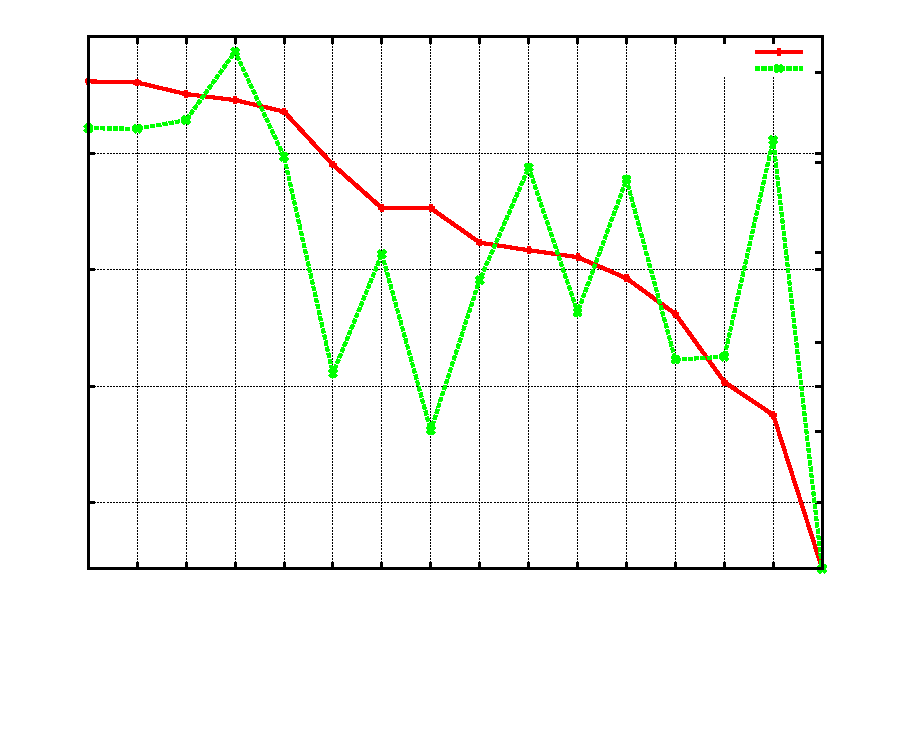
\includegraphics{plots/seq2}}%
    \gplfronttext
  \end{picture}%
\endgroup
}
% GNUPLOT: LaTeX picture with Postscript
\begingroup
  \makeatletter
  \providecommand\color[2][]{%
    \GenericError{(gnuplot) \space\space\space\@spaces}{%
      Package color not loaded in conjunction with
      terminal option `colourtext'%
    }{See the gnuplot documentation for explanation.%
    }{Either use 'blacktext' in gnuplot or load the package
      color.sty in LaTeX.}%
    \renewcommand\color[2][]{}%
  }%
  \providecommand\includegraphics[2][]{%
    \GenericError{(gnuplot) \space\space\space\@spaces}{%
      Package graphicx or graphics not loaded%
    }{See the gnuplot documentation for explanation.%
    }{The gnuplot epslatex terminal needs graphicx.sty or graphics.sty.}%
    \renewcommand\includegraphics[2][]{}%
  }%
  \providecommand\rotatebox[2]{#2}%
  \@ifundefined{ifGPcolor}{%
    \newif\ifGPcolor
    \GPcolortrue
  }{}%
  \@ifundefined{ifGPblacktext}{%
    \newif\ifGPblacktext
    \GPblacktexttrue
  }{}%
  % define a \g@addto@macro without @ in the name:
  \let\gplgaddtomacro\g@addto@macro
  % define empty templates for all commands taking text:
  \gdef\gplbacktext{}%
  \gdef\gplfronttext{}%
  \makeatother
  \ifGPblacktext
    % no textcolor at all
    \def\colorrgb#1{}%
    \def\colorgray#1{}%
  \else
    % gray or color?
    \ifGPcolor
      \def\colorrgb#1{\color[rgb]{#1}}%
      \def\colorgray#1{\color[gray]{#1}}%
      \expandafter\def\csname LTw\endcsname{\color{white}}%
      \expandafter\def\csname LTb\endcsname{\color{black}}%
      \expandafter\def\csname LTa\endcsname{\color{black}}%
      \expandafter\def\csname LT0\endcsname{\color[rgb]{1,0,0}}%
      \expandafter\def\csname LT1\endcsname{\color[rgb]{0,1,0}}%
      \expandafter\def\csname LT2\endcsname{\color[rgb]{0,0,1}}%
      \expandafter\def\csname LT3\endcsname{\color[rgb]{1,0,1}}%
      \expandafter\def\csname LT4\endcsname{\color[rgb]{0,1,1}}%
      \expandafter\def\csname LT5\endcsname{\color[rgb]{1,1,0}}%
      \expandafter\def\csname LT6\endcsname{\color[rgb]{0,0,0}}%
      \expandafter\def\csname LT7\endcsname{\color[rgb]{1,0.3,0}}%
      \expandafter\def\csname LT8\endcsname{\color[rgb]{0.5,0.5,0.5}}%
    \else
      % gray
      \def\colorrgb#1{\color{black}}%
      \def\colorgray#1{\color[gray]{#1}}%
      \expandafter\def\csname LTw\endcsname{\color{white}}%
      \expandafter\def\csname LTb\endcsname{\color{black}}%
      \expandafter\def\csname LTa\endcsname{\color{black}}%
      \expandafter\def\csname LT0\endcsname{\color{black}}%
      \expandafter\def\csname LT1\endcsname{\color{black}}%
      \expandafter\def\csname LT2\endcsname{\color{black}}%
      \expandafter\def\csname LT3\endcsname{\color{black}}%
      \expandafter\def\csname LT4\endcsname{\color{black}}%
      \expandafter\def\csname LT5\endcsname{\color{black}}%
      \expandafter\def\csname LT6\endcsname{\color{black}}%
      \expandafter\def\csname LT7\endcsname{\color{black}}%
      \expandafter\def\csname LT8\endcsname{\color{black}}%
    \fi
  \fi
  \setlength{\unitlength}{0.0500bp}%
  \begin{picture}(8502.00,6802.00)%
    \gplgaddtomacro\gplbacktext{%
      \csname LTb\endcsname%
      \put(592,1988){\makebox(0,0)[r]{\strut{} 77}}%
      \csname LTb\endcsname%
      \put(592,2618){\makebox(0,0)[r]{\strut{} 80}}%
      \csname LTb\endcsname%
      \put(592,3248){\makebox(0,0)[r]{\strut{} 83}}%
      \csname LTb\endcsname%
      \put(592,3878){\makebox(0,0)[r]{\strut{} 86}}%
      \csname LTb\endcsname%
      \put(592,4509){\makebox(0,0)[r]{\strut{} 89}}%
      \csname LTb\endcsname%
      \put(592,5139){\makebox(0,0)[r]{\strut{} 92}}%
      \csname LTb\endcsname%
      \put(592,5769){\makebox(0,0)[r]{\strut{} 95}}%
      \csname LTb\endcsname%
      \put(592,6399){\makebox(0,0)[r]{\strut{} 98}}%
      \csname LTb\endcsname%
      \put(688,1408){\rotatebox{-270}{\makebox(0,0)[r]{\strut{}\relu}}}%
      \csname LTb\endcsname%
      \put(1151,1408){\rotatebox{-270}{\makebox(0,0)[r]{\strut{}\lrelua}}}%
      \csname LTb\endcsname%
      \put(1615,1408){\rotatebox{-270}{\makebox(0,0)[r]{\strut{}\swish}}}%
      \csname LTb\endcsname%
      \put(2078,1408){\rotatebox{-270}{\makebox(0,0)[r]{\strut{}\pentan}}}%
      \csname LTb\endcsname%
      \put(2541,1408){\rotatebox{-270}{\makebox(0,0)[r]{\strut{}\lrelub}}}%
      \csname LTb\endcsname%
      \put(3004,1408){\rotatebox{-270}{\makebox(0,0)[r]{\strut{}\arctid}}}%
      \csname LTb\endcsname%
      \put(3468,1408){\rotatebox{-270}{\makebox(0,0)[r]{\strut{}\elu}}}%
      \csname LTb\endcsname%
      \put(3931,1408){\rotatebox{-270}{\makebox(0,0)[r]{\strut{}\minsin}}}%
      \csname LTb\endcsname%
      \put(4394,1408){\rotatebox{-270}{\makebox(0,0)[r]{\strut{}\maxtanh}}}%
      \csname LTb\endcsname%
      \put(4857,1408){\rotatebox{-270}{\makebox(0,0)[r]{\strut{}\mytanh}}}%
      \csname LTb\endcsname%
      \put(5321,1408){\rotatebox{-270}{\makebox(0,0)[r]{\strut{}\mysin}}}%
      \csname LTb\endcsname%
      \put(5784,1408){\rotatebox{-270}{\makebox(0,0)[r]{\strut{}\maxsig}}}%
      \csname LTb\endcsname%
      \put(6247,1408){\rotatebox{-270}{\makebox(0,0)[r]{\strut{}\selu}}}%
      \csname LTb\endcsname%
      \put(6710,1408){\rotatebox{-270}{\makebox(0,0)[r]{\strut{}\linear}}}%
      \csname LTb\endcsname%
      \put(7174,1408){\rotatebox{-270}{\makebox(0,0)[r]{\strut{}\sigmoid}}}%
      \csname LTb\endcsname%
      \put(7637,1408){\rotatebox{-270}{\makebox(0,0)[r]{\strut{}\cosid}}}%
      \put(7733,1534){\makebox(0,0)[l]{\strut{} 30}}%
      \put(7733,2259){\makebox(0,0)[l]{\strut{} 40}}%
      \put(7733,2984){\makebox(0,0)[l]{\strut{} 50}}%
      \put(7733,3709){\makebox(0,0)[l]{\strut{} 60}}%
      \put(7733,4434){\makebox(0,0)[l]{\strut{} 70}}%
      \put(7733,5159){\makebox(0,0)[l]{\strut{} 80}}%
      \put(7733,5884){\makebox(0,0)[l]{\strut{} 90}}%
      \put(7733,6609){\makebox(0,0)[l]{\strut{} 100}}%
      \put(128,4056){\rotatebox{-270}{\makebox(0,0){\strut{}Score}}}%
    }%
    \gplgaddtomacro\gplfronttext{%
      \csname LTb\endcsname%
      \put(6902,6466){\makebox(0,0)[r]{\strut{}\best}}%
      \csname LTb\endcsname%
      \put(6902,6306){\makebox(0,0)[r]{\strut{}\avg}}%
    }%
    \gplbacktext
    \put(0,0){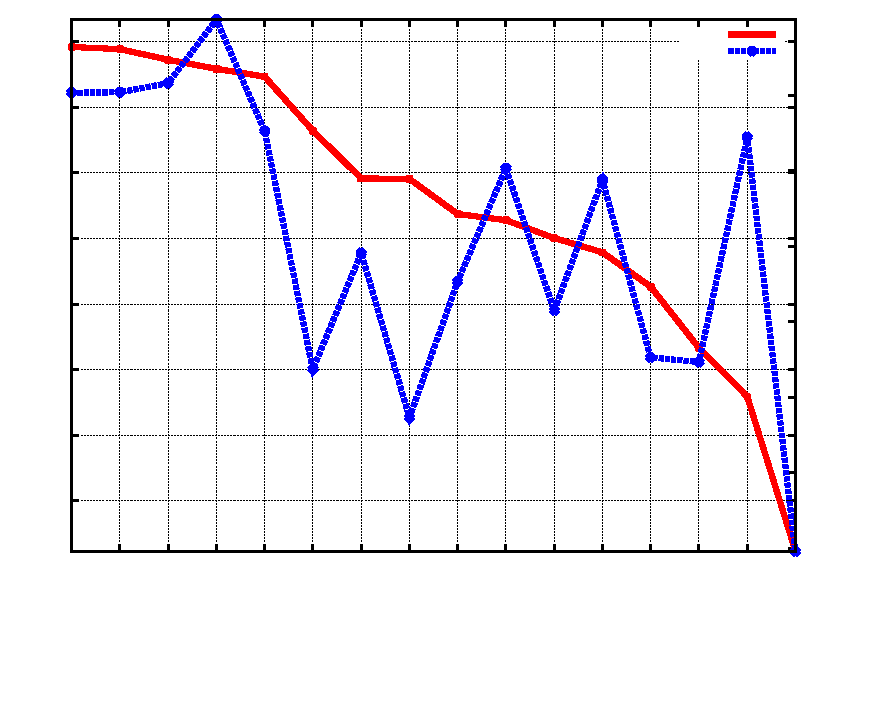
\includegraphics{plots/seq-X.pdf}}%
    \gplfronttext
  \end{picture}%
\endgroup
}
\caption{Sequence tagging.}
\label{fig:seq}
\end{figure}

Unlike for sentence classification, there are much larger differences between the activation functions. For example, there is almost 20pp difference between the best \best{} activation functions: \relu{}, \lrelua{}, \swish{}, \pentan{}, and the worst ones: \linear{}, \cosid{}, and \sigmoid{} (the differences were larger had we included \cube{}). Interestingly, this difference is mostly due to the TL-AM task: for POS, there is only 3pp difference between the best function (\sigmoid{} (sic!), though with almost zero margin to the next best ones) and the worst one (\linear), while this difference is almost 40pp for TL-AM. 
%If we follow conventional wisdom, then we would speculate that POS tagging is a too simple task where the label for a token only depends on the current token and some small context. Thus, the task apparently lacks long-range dependencies, as we had reasoned, which may cause different activation functions to have little influence on performance.
This appears to confirm our concerns regarding the POS tagging task as not being challenging enough due to lack of, e.g., long-range dependencies.

The four best \best{} activation functions in Figure \ref{fig:seq} are also the functions with the best \avg{} results, i.e., they are most stable over different hyperparameters. %choices. 
The clear winner in this category is \pentan{} with 100\% \avg{} score, followed by \swish{} with 91\%. Worst is \cosid{} with 30\%. It is remarkable how large the difference between \mytanh{} and \pentan{} is both for \best{} and \avg{}---7pp and 20pp, respectively, which is much larger than the differences between the analogous pair of LReLU and \relu{}. This appears to make a strong case for the importance of the slope around the origin, as suggested in \citet{Xu:2016}. 
%, lacking, e.g., long-range dependencies  

%\begin{table}[!htb]
%  \centering
%  \begin{tabular}{lrr}
%    \toprule
%    Function & Best & Avg \\ \midrule
%    \relu & 52.95 \\
%    \lrelua & 52.92 \\
%    \swish & 52.66 \\
%    \lrelub & 52.19 \\
%    \pentan & 51.76 \\
%    \arctid & 50.23 \\
%    \midrule
%    \elu & 48.72 \\
%    \minsin & 48.43 \\
%    \maxtanh & 47.42 \\
%    \mytanh & 46.74 \\
%    \mysin & 46.00 \\
%    \maxsig & 45.54 & \\
%    \selu & 44.72 & \\
%    \linear & 42.20 & \\
%    \midrule
%    \sigmoid & 39.58 & \\
%    \cosid & 34.76 & \\
%    \cube & 11.33 & \\
%  \end{tabular}
%  \caption{ArgMin PE, macro-F1 scores %in \%.}
%  \label{table:seq_pe}
%\end{table}

\paragraph{LSTM vs.\ RNN} Besides an RNN, we also implemented a more popular RNN model with (bidirectional) LSTM blocks in place of standard hidden layers. Standard LSTM units follow the equations (simplified):
\begin{align*}
  \mathbf{f}_t &= \sigma([\mathbf{h}_{t-1};\mathbf{x}_t]\cdot \mathbf{W}_f),\\
  \mathbf{i}_t &= \sigma([\mathbf{h}_{t-1};\mathbf{x}_t]\cdot \mathbf{W}_i),\\
  %&\vdots \\
  \mathbf{o}_t &= \sigma([\mathbf{h}_{t-1};\mathbf{x}_t]\cdot \mathbf{W}_o)\\
  \mathbf{c}_t &= \mathbf{f}_t\odot \mathbf{c}_{t-1}+\mathbf{i}_t\odot\tau([\mathbf{h}_{t-1};\mathbf{x}_t]\cdot \mathbf{W}_c)\\
  \mathbf{h}_t &= \mathbf{o}_t\odot \tau(\mathbf{c}_t),
\end{align*}
where $\mathbf{f}_t$ and $\mathbf{i}_t$ are perceived of as \emph{gates} that control information flow,
%(further gates and equations skipped for readability), 
$\mathbf{x}_t$ is the input at time $t$ and $\mathbf{h}_t$ is the hidden layer activation. In keras (and most standard references), $\sigma$ is the (hard) sigmoid function, and $\tau$ is the \mytanh{} function. 

We ran an LSTM on the TL-AM dataset with Levy word embeddings and 5\% and 30\% data size setup. We varied $\sigma$ and $\tau$ independently, keeping the respective other function at its default. 

We find that the top two choices for $\tau$ are \pentan{} and \mytanh{} (margin of 10pp), given that $\sigma$ is sigmoid. For $\tau=$ \mytanh{}, the best choices are $\sigma=$ \pentan{}, \sigmoid, and \mytanh{}. All other functions perform considerably worse. Thus, the top-performers are all saturating functions, indicating the different roles activation functions play in LSTMs---those of gates---compared to standard layers. It is worth mentioning that choosing $\sigma$ or $\tau$ as \pentan{} is on average better than the standard choices for $\sigma$ and $\tau$. %[Moreover, when we choose both $\sigma$ and $\tau$ as \pentan{}, then ...]
Indeed, choosing $\tau=\sigma=$ \pentan{} is on average 2pp better than the default choices of $\tau,\sigma$.
%and is on par with the choice $\tau=$ \sigmoid{} and $\sigma=$ \pentan{}. 

It is further worth mentioning that the best \best{} results for the LSTM are roughly 5pp better (absolute) than the best corresponding choices for the simple RNN. 

